\chapter{Analisi 0}
Questo capitolo contiene alcuni argomenti che non fanno parte del programma di Analisi Matematica ma che possono essere utili alla comprensione degli argomenti.

\section{Disequazioni}
Nel corso di Analisi Matematica troviamo spesso delle disequazioni da risolvere, è bene quindi sapere come risolverle.

\paragraph*{Le disequazioni} sono come delle equazioni in cui ci si chiede "per quali valori di $x$ questa espressione è maggiore (minore) di un certo valore".
Vengono risolte esattamente come le equazioni, ma il significato del risultato è diverso.
\subsection*{Disequazioni Fratte e con Prodotti di Polinomi}
Le disequazioni in forma fratta o prodotti, quindi in forma $\frac{P}{D}>0$ o $(P)(D)>0$ con $P,D$ Polinomi si risolvono semplicemente \emph{studiando il segno dei due fattori e unendo il risultato}.
\esempio{$(x-2)(x+1) \geq 0$
\\Studio il segno del primo membro: $(x-2)\geq 0 \to x\geq 2$
\\E del secondo membro: $(x+1) \geq 0 \to x\geq -1$.
Facendo il grafico dei segni ottengo:
\\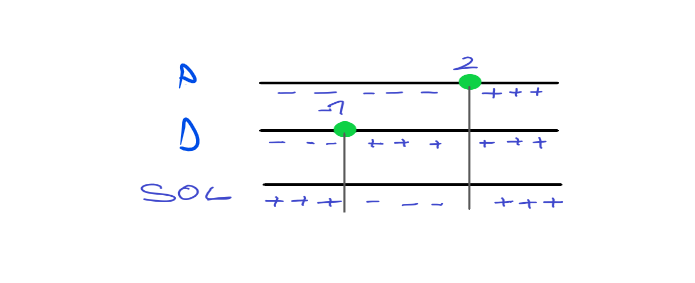
\includegraphics[width=\textwidth]{esempio-disequaz-prodotto.png}
\\Di conseguenza, la soluzione della disequazione è: $S= (-\infty,-1]\cup[2,+\infty)$
} 
\nb{
	Per le \emph{disequazioni fratte}, \textbf{il denominatore non può mai essere uguale a zero},
	quindi deve essere \textbf{strettamente maggiore (minore)}.
}
\subsection*{Disequazioni di secondo grado}
Le disequazioni (come le equazioni) di secondo grado si risolvono, una volta ridotte alla forma standard $ax^2+bx+c$, usando la formula risolutiva:
\[ x_{1 2} = \frac{-b\pm\sqrt{b^2-4ac}}{2a} \]
\paragraph*{Formula Ridotta}
Quando il \emph{coefficiente di primo grado è pari} è possibile applicare la seguente forumula detta \textbf{ridotta}:
\[ x_{1,2} = \frac{-\frac{b}{2}\pm \sqrt{\frac{b}{2}}^2 - ac}{a} \]

A seconda del valore di $\Delta = b^2-4ac$, la disequazione (equazione) ammette:
\begin{itemize}
	\item $\Delta > 0 \implies $ 2 soluzioni Reali
	\item $\Delta < 0 \implies $ Nessuna soluzione Reale (ma 2 complesse)
	\item $\Delta = 0 \implies $ 1 Soluzione Reale (2 soluzioni coincidenti)
\end{itemize}
Ricordiamo poi, che un'equazione del tipo $y=ax^2 +bx +c$ è una \emph{parabola}, quindi con una disequazione (ponendo $f(x)>0$) ci si chiede semplicemente per quali valori di $x$ la funzione è maggiore di 0,
quindi quando sta sopra l'asse delle ascisse.


Il $\Delta$, e il valore del parametro $a$ della funzione determinano la "rappresentazione" della parabola
\\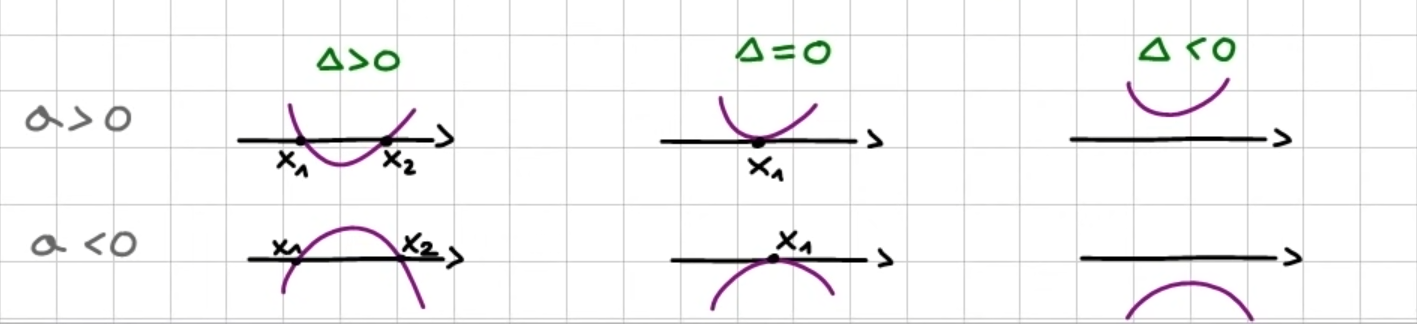
\includegraphics[width=\textwidth]{parabole-delta.png}

\paragraph*{Tabella delle soluzioni} Questa tabella è utile a capire quali sono le soluzioni di una disequazione.
\\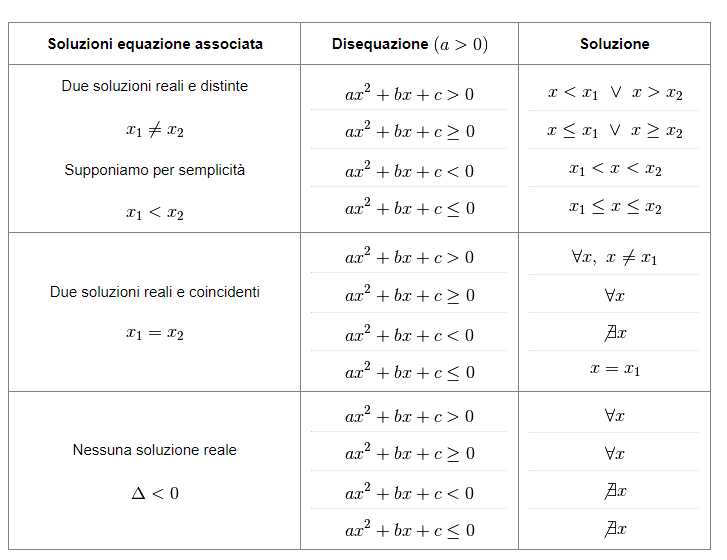
\includegraphics[width=\textwidth]{disequazioni.png}


\subsection*{Disequazioni con \emph{Valore Assoluto}}
Quando troviamo una disequazione con valore assoluto, bisogna porre a sistema la disequazione con \emph{l'argomento del modulo posto prima maggiore, poi minore di zero}.
Così facendo avremo due sistemi di disequazioni, che risolti separatamente ci daranno i due risultati della disequazione
\subparagraph{in parole più semplici} Noi vogliamo vedere la soluzione della disequazione con l'argomento del modulo sia "così com'è" che con i segni invertiti e poi unire i risultati.
Quindi il risultato del modulo posto maggiore o minore di zero non ci interessa! 
\nb{(\textbf{non sono sicuro} di questo ragionamento. per ora diamolo per buono )}

\esempio{
	$|2x-3| > x + 6$. Dobbiamo eliminare il valore assoluto.
	\\quindi ponendo l'argomento del modulo \emph{maggiore o uguale a zero}:
	\begin{equation*}
		\begin{cases}
			2x-3 \geq 0 \\
			2x-3 > x+6
		\end{cases}
		=
		\begin{cases}
			x\geq \frac{3}{2}\\
			x > 9
		\end{cases}
		= x>9
	\end{equation*}
	E ponendolo \emph{minore di zero} (nota che cambia di segno):
	\begin{equation*}
		\begin{cases}
			2x-3 < 0 \\
			-2x+3 > x+6
		\end{cases}
		=
		\begin{cases}
			x < \frac{3}{2}\\
			x < -1
		\end{cases}
		= x<-1
	\end{equation*}
	Quindi il risultato è: $x>9 \vee x<-1$
}
Nel caso in cui avessi un valore assoluto dentro un altro parto sempre da quello più
esterno a definire le condizioni e creare i sistemi.
\\ Quando ottengo che una soluzione di un sistema non esiste posso
non considerarla nell'unione finale delle varie soluzioni dei sistemi. 

\section{Richiamo sui Logaritmi}
\definizione{
	Il logaritmo è un operatore matematico indicato generalmente con $\log_a(b)$;
	\\Detta $a$ la base e $b$ l'argomento, il logaritmo in base a di b è definito come:
	\begin{center}
		\emph{L'esponente a cui elevare la base per ottenere l'argomento.}
	\end{center}
	$$\log_a(b)=c \implies a^c=b$$
	\\ Il logaritmo è l'operazione inversa rispetto all'elevamento a potenza.
	}
	\begin{center}
		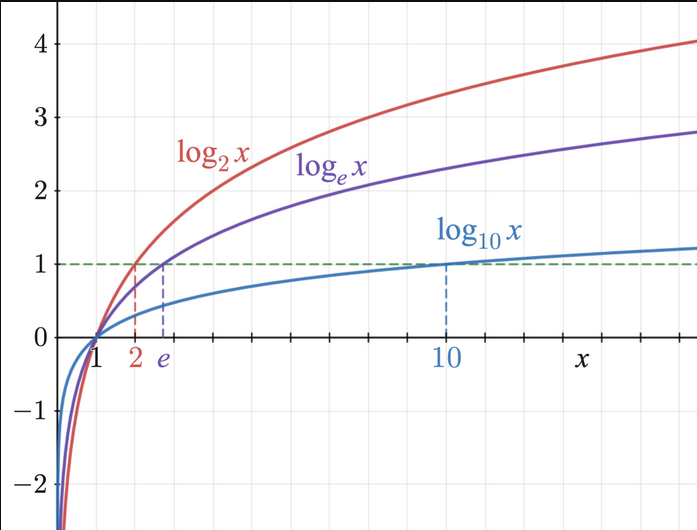
\includegraphics[width=70mm, scale=0.5]{logaritmi-grafico.png}
		\end{center}
\subsection*{Proprietà dei logaritmi}
Per i logaritmi valgono le seguenti prorpietà:
\begin{itemize}
	\item Toerema del prodotto: $\log_a(b\cdot c) = \log_a(b) + \log_a(c)$
	\item Teorema del rapporto: $\log_a(\frac{b}{c})= \log_a(b) - \log_a(c)$
	\item Regola dell'esponente: $\log_a(b^c) = c \log_a(b)$
	\item Formula del cambiamento di base : $\log_a(b) = \frac{\log_c(b)}{\log_c(a)}$
	\item Formula di inversione : $\log_a(b) = \frac{1}{\log_b(a)}$
\end{itemize}


\paragraph*{Condizioni di esistenza} Durante la risoluzione di una disequazione dobbiamo ricordarci
di porre come condizione di esistenza l'argomento del logaritmo maggiore di 0, come si può osservare dal grafico
il logaritmo non assume mai 0 come valore sull'asse delle x.
\section{Richiamo di Trigonometria}

\paragraph*{Seno e Coseno}
Due funzioni trigonometriche fondamentali sono \emph{Seno e Coseno}, che vengono definite
a partire dalla circonferenza goniometrica e che \emph{associa a ciascun angolo un determinato
valore numerico compreso tra -1 e +1}.
\\Le seguenti immagini evidenziano il significato geometrico del seno e del coseno:
\begin{center}
	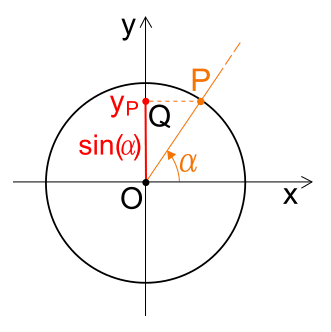
\includegraphics[width=50mm, scale=0.5]{seno_geom.png}
	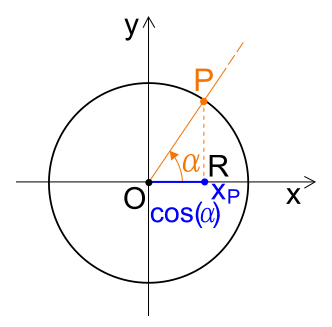
\includegraphics[width=50mm, scale=0.5]{coseno_geom.png}
\end{center}
\paragraph*{Tangente} Sempre partendo dalla circonferenza goniometrica possiamo definire la
tangente di un angolo come il rapporto tra il seno e il coseno dello stesso angolo.
\\ Qui di seguito il significato geometrico della tangente.
\begin{center}
	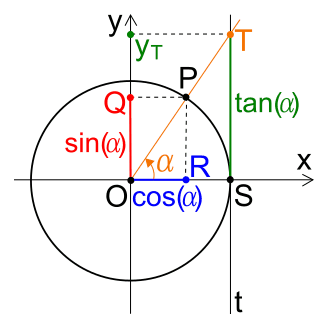
\includegraphics[width=50mm, scale=0.5]{tangente_geom.png}
\end{center}

\paragraph*{Valori di Seno e Coseno} Al variare di $\alpha$
\\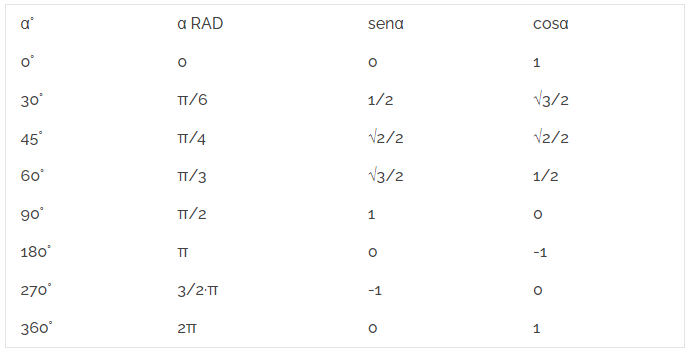
\includegraphics[width=\textwidth]{senocoseno.png}

\paragraph*{Formule Note}
Seguono alcune formule trigonometriche note che possono essere utili durante gli esami.
\begin{itemize}
	\item $\frac{\sin(x)}{\cos(x)} = \tan(x)$
	\item $\frac{\cos(x)}{\sin(x)} = \frac{1}{\tan(x)} = \cot(x)$
\end{itemize}

\paragraph*{Proprietà}
\begin{itemize}
	\item $\sin(\alpha + \beta) = sin(\alpha) + \sin(\beta)$
\end{itemize}
\section{Valore assoluto (modulo) di un numero Reale}
\paragraph*{Definizione Valore assoluto} Il \textbf{valore assoluto}, detto anche \emph{modulo}, è una funzione che
associa ad un numero negativo il numero stesso con segno positivo, a zero associa zero e lascia invariati i 
numeri positivi. 
\definizione{ Per ogni $x \in R$ si pone
	\begin{equation}
		|x| = \begin{cases}
			x  & \text{se $x \geq 0$} \\
			-x & \text{se $x < 0$}
		\end{cases}
	\end{equation}
	$|x|$ si dice valore assoluto, o modulo, di x
}
Il valore assoluto di un numero è quindi \textbf{sempre positivo o eventualmente nullo}. 
\paragraph{ATTENZIONE} dire che "il modulo di un numero è il numero senza il segno" non ha senso in questo contesto, quindi non va usata perchè vale solo se x è "semplice"
\paragraph{In parole povere} il modulo di $x$ è $x$ se x è positivo, il suo opposto se è negativo\\
quindi $|3 - \pi| = \pi - 3$ perchè $3-\pi$ è negativo ($3 - 3.14$) quindi il suo modulo è il suo opposto.
\\Volendo, $|x|$ si può anche interpretare come il massimo tra $x$ e $-x$.

\paragraph{Modulo e moltiplicazione}
Per ogni $x, y \in R$ si ha $|xy| = |x||y|$.\\Se $y\neq0$, si ha anche $|x/y|=|x|/|y|$
\paragraph{Modulo e addizione}
Il modulo della somma NON coincide con la somma dei moduli. Però vale la seguente importantissima disuguaglianza:
\paragraph{Disuguaglianza triangolare} siano x,y numeri reali. Allora:
\begin{equation}
	|x+y| \leq |x| + |y|
\end{equation}
(cioè il modulo della somma è minore o uguale della somma dei due moduli)

\section{Insiemi e Intervalli in R}
\definizione{
	Diremo \textbf{intervallo} di $\R$ un sottoinsieme $I$ di $\R$ che sia convesso rispetto all'ordine, cioè che soddisfi la seguente condizione:
	se $a,b \in I$, e $a \leq b$, ogni $x\in R$ tale che $a \leq x \leq b$ appartiene a $I$.
}

In parole povere: $I$ è intervallo di $\R$ se, contenendo due numeri reali, contiene anche \emph{tutti i numeri reali che stanno fra questi due}.

\paragraph{Intervalli limitati.}
Fissati $a, b \in R$, con $a<b$, si riconosce facilmente che sono intervalli i seguenti sottoinsiemi di $\R$:
\begin{itemize}
	\item[] $[a,b] = \{x \in R : a \leq x \leq b\}$ CHIUSO
	\item[] $[a,b) = \{x \in R : a \leq x < b\}$ SUPERIORMENTE APERTO
	\item[] $(a,b] = \{x \in R : a < x \leq b\}$ INFERIORMENTE APERTO
	\item[] $(a,b) = \{x \in R : a < x < b\}$ APERTO
\end{itemize}
{\tiny(le parentesi tonde a volte vengono sostituite con delle parentesi quadre nel senso opposto)}
\\Tutti questi intervalli sono detti intervalli \emph{limitati}
\paragraph{Intervalli illimitati.} sono invece intervalli illimitati, per ogni $a \in R$, gli insiemi:
\begin{itemize}
	\item[] $\{x \in R: x \geq a\}$ (semiretta \emph{chiusa} inferiormente limitata)
	\item[] $\{x \in R: x > a\}$ (semiretta \emph{aperta} inferiormente limitata)
	\item[] $\{x \in R: x \leq a\}$ (semiretta \emph{chiusa} superiormente limitata)
	\item[] $\{x \in R: x < a\}$ (semiretta \emph{aperta} superiormente limitata)
\end{itemize}

\subsection*{Massimi e Minimi dei sottoinsiemi di $\R$}
\paragraph{Definizione.} Sia $S$ un sottoinsieme di $\R$. Un elemento $m\in R$ si dice \emph{massimo} di S se appartiene ad S ed è maggiore o uguale di ogni elemento di $S$.
\\Dualmente, $\mu \in \R $ è detto \emph{minimo} di $S$ se appartiene ad $S$ ed è minore o uguale di ogni elemento di $S$
\\Un sottoinsieme può \emph{avere o non avere massimo}, \emph{avere o non avere minimo}, ma se esistono sono \textbf{UNICI}.

\paragraph*{Maggioranti/Minoranti}
Un numero reale L si dice \textbf{maggiorante} per un insieme A di numeri reali se è maggiore o uguale di ogni elemento di A.
\\In simboli: $L$ è maggiorante di $A$ $\Leftrightarrow L\geq a, \forall a \in A$
\\Viceversa vale per i \textbf{Minoranti}.
\subparagraph*{insiemi limitati} Se un insieme ammette maggioranti, allora si dice che è \emph{Superiormente limitato}, viceversa per i minoranti.
Se un insieme ammette sia maggioranti che minoranti, allora esso è limitato.

% \paragraph{Definizioni.} Sia $S$ sottoinsieme non vuoto di $\R$. si dice che $b\in \R$ è un \emph{maggiorante} per $S$ se risulta $s\leq b$ per ogni $s \in S$. Si dice che $S$ è \emph{Superiormente limitato} (in $\R$) se ammette maggioranti in $\R$.
% \\l'insieme dei maggioranti in $\R$ di $S\subseteq \R$ è indicato con $S^*$.
% \\dualmente per i minoranti, ovviamente i minoranti sono tutti minori di $S$ e l'insieme dei minoranti si indica con $S_*$.
% \\Un insieme non vuoto $S \subseteq \R$ si dice \emph{limitato} se è tanto superiormente limitato quanto inferiormente limitato.
\paragraph*{In parole povere} Un Massimo è un numero compreso nell'insieme che è più grande di tutti gli altri, un maggiorante è un numero (che può essere compreso o non) che è maggiore o uguale a tutti gli altri. 
\subsection*{Prodotto Cartesiano}
\paragraph{Definizione.}Dati due insiemi $X$ e $Y$, il loro prodotto cartesiano è per definizione l'insieme $X \times Y$ formato da tutte le coppie ordinate $(x,y)$ che hanno la prima componente $x \in X$, la seconda $y \in Y$.\\
Se $X = Y$, il prodotto $X \times X$ si chiama \emph{quadrato cartesiano} di $X$ e si indica anche con $X^2$
